% ══════════════════════════════════════════════════════════════════════════════
%  bench_spatial_kernels.tex
%  VSEPR-SIM Benchmark Suite — Layer 2
%  Direct O(N²) VSEPR Field Kernel vs Simulation-Side Octree
%
%  Compile:  pdflatex bench_spatial_kernels.tex   (twice for TOC / refs)
%            or: latexmk -pdf bench_spatial_kernels.tex
%
%  Part of the FlowerOS HPC stack  (docs/bench_spatial_kernels.tex)
% ══════════════════════════════════════════════════════════════════════════════

\documentclass[11pt,a4paper]{article}

% ── packages ──────────────────────────────────────────────────────────────────
\usepackage[utf8]{inputenc}
\usepackage[T1]{fontenc}
\usepackage{lmodern}
\usepackage[margin=2.4cm]{geometry}
\usepackage{amsmath,amssymb,amsthm}
\usepackage{graphicx}
\usepackage{xcolor}
\usepackage{booktabs}
\usepackage{enumitem}
\usepackage{listings}
\usepackage{hyperref}
\usepackage{tikz}
\usetikzlibrary{arrows.meta,positioning,fit,calc,shapes.geometric,trees}

% ── colours (FlowerOS pastel palette) ─────────────────────────────────────────
\definecolor{fosMint}{HTML}{87CEEB}
\definecolor{fosMagenta}{HTML}{D8A0D8}
\definecolor{fosGreen}{HTML}{87D687}
\definecolor{fosYellow}{HTML}{F0E68C}
\definecolor{fosGrey}{HTML}{A0A0A0}
\definecolor{fosBlue}{HTML}{6495ED}
\definecolor{fosOrange}{HTML}{FFA07A}
\definecolor{fosCode}{HTML}{F5F5F5}

\hypersetup{
  colorlinks=true,
  linkcolor=fosBlue,
  citecolor=fosBlue,
  urlcolor=fosMint,
  pdftitle={VSEPR Benchmark Layer 2 -- Spatial Kernels},
  pdfauthor={FlowerOS Project},
}

% ── listings style ────────────────────────────────────────────────────────────
\lstset{
  basicstyle=\ttfamily\small,
  backgroundcolor=\color{fosCode},
  frame=single,
  framerule=0.4pt,
  rulecolor=\color{fosGrey},
  keywordstyle=\color{fosBlue}\bfseries,
  commentstyle=\color{fosGrey}\itshape,
  stringstyle=\color{fosOrange},
  showstringspaces=false,
  breaklines=true,
  language=C++,
}

% ── theorem-like environments ─────────────────────────────────────────────────
\theoremstyle{definition}
\newtheorem{definition}{Definition}[section]
\newtheorem{contract}[definition]{Contract}
\theoremstyle{plain}
\newtheorem{proposition}[definition]{Proposition}

% ── macros ────────────────────────────────────────────────────────────────────
\newcommand{\Nq}{N_{\mathrm{pairs}}}
\newcommand{\Otwo}{\mathcal{O}(N^2)}
\newcommand{\OnlogN}{\mathcal{O}(N \log N)}
\newcommand{\rcut}{r_{\mathrm{cut}}}
\newcommand{\eps}{\varepsilon}

% ── title ─────────────────────────────────────────────────────────────────────
\title{%
  \textbf{VSEPR-SIM Benchmark Suite} \\[4pt]
  \Large Layer 2: Spatial Kernel Performance Comparison \\[14pt]
  \normalsize Direct $\mathcal{O}(N^2)$ VSEPR Field Kernel
  \quad vs \quad Simulation-Side Octree%
}
\author{FlowerOS Project}
\date{v5.0.14 \quad \today}

% ══════════════════════════════════════════════════════════════════════════════
\begin{document}
\maketitle
\thispagestyle{empty}

\begin{abstract}
This document describes \textbf{Layer~2} of the VSEPR-SIM benchmark suite:
a correctness-validated timing comparison between the preexisting
$\mathcal{O}(N^2)$ all-pairs VSEPR nonbonded field kernel and a newly
implemented simulation-side octree with AABB-pruned leaf-pair traversal.
Both paths evaluate identical LJ-12-6 energy; a per-run $\Delta E$ column
acts as an end-to-end correctness gate.  Metrics include octree build time
(separate from evaluation time), number of pairs evaluated, energy value,
speedup factor, and $\Delta E$.
The benchmark is self-contained (stdlib only, no GLM or VSEPR headers) and
covers log-spaced atom counts $N \in [64, 4096]$.
\end{abstract}

\tableofcontents
\newpage

% ──────────────────────────────────────────────────────────────────────────────
\section{Background and Motivation}
\label{sec:background}

\subsection{The O(N²) Wall}

The VSEPR nonbonded kernel (\texttt{src/pot/energy\_nonbonded.hpp}) evaluates
every distinct atom pair $(i, j)$ with $i < j$:
\begin{equation}
  U = \sum_{i < j} s_{ij}\,U_{\mathrm{LJ}}(r_{ij})
  \label{eq:direct-sum}
\end{equation}
where $s_{ij}$ is a 1-2/1-3/1-4 topology scaling factor.
The number of pair evaluations scales as $\Nq = N(N-1)/2$, giving
$\Otwo$ cost per energy/force call.  For $N = 1000$ this is $499\,500$
pair evaluations; for $N = 4096$ it grows to over $8 \times 10^6$.

A comment in \texttt{tests/pbc\_phase4\_perf.cpp} notes that
\emph{after adding neighbor lists, throughput should improve $\sim$10--100$\times$}.
This benchmark provides the empirical baseline for that claim.

\subsection{Spatial Acceleration via Octrees}

An octree recursively subdivides space into eight octants, grouping nearby
atoms into leaf nodes.  For a pair cutoff $\rcut$, two leaf nodes whose
axis-aligned bounding boxes (AABBs) are separated by more than $\rcut$ can
be skipped entirely — reducing the effective pair count from $\Otwo$ toward
$\mathcal{O}(N)$ in sparse, well-separated systems.

\begin{figure}[ht]
\centering
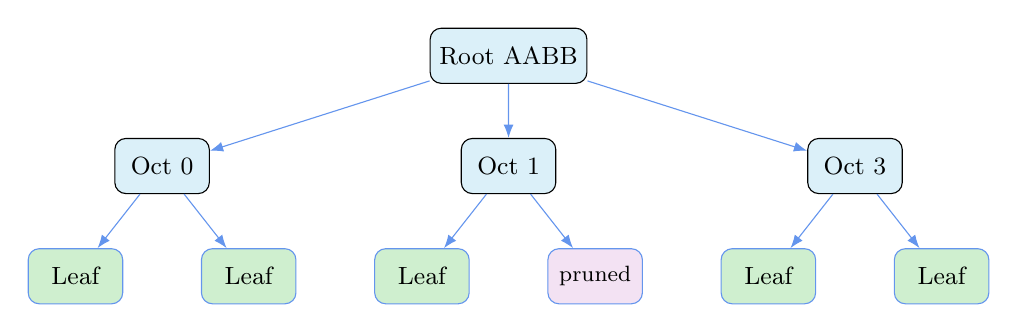
\begin{tikzpicture}[
  level 1/.style={sibling distance=44mm,level distance=14mm},
  level 2/.style={sibling distance=22mm,level distance=14mm},
  every node/.style={draw,rounded corners,
					 minimum width=12mm, minimum height=7mm,
					 fill=fosMint!30, font=\small},
  edge from parent/.style={draw,fosBlue,-Latex},
]
\node {Root AABB}
  child { node {Oct 0}
	child { node[fill=fosGreen!40] {Leaf} }
	child { node[fill=fosGreen!40] {Leaf} }
  }
  child { node {Oct 1}
	child { node[fill=fosGreen!40] {Leaf} }
	child { node[fill=fosMagenta!30] {\footnotesize pruned} }
  }
  child { node {Oct 3}
	child { node[fill=fosGreen!40] {Leaf} }
	child { node[fill=fosGreen!40] {Leaf} }
  };
\end{tikzpicture}
\caption{Schematic octree: leaf nodes (green) are evaluated pairwise;
  grey (magenta) nodes whose AABB is $> \rcut$ from all query nodes are
  pruned without atom-level work.}
\label{fig:octree}
\end{figure}

\subsection{Scope of this Benchmark}

The simulation octree implemented here is entirely separate from the
rendering \texttt{OctreeNode} in \texttt{include/render/scalable\_renderer.hpp},
which uses GLM and is designed for frustum culling only.
The benchmark octree uses only the C++ standard library and is purpose-built
for simulation pair queries.

% ──────────────────────────────────────────────────────────────────────────────
\section{Force Field: Shared LJ-12-6 Kernel}
\label{sec:ff}

Both kernels evaluate the truncated Lennard-Jones potential:
\begin{equation}
  U_{\mathrm{LJ}}(r) = \begin{cases}
	4\eps\left[(\sigma/r)^{12} - (\sigma/r)^{6}\right]
	  & r < \rcut \\
	0 & r \ge \rcut
  \end{cases}
  \label{eq:lj}
\end{equation}
with Ar-like parameters:
\begin{center}
\begin{tabular}{lll}
\toprule
Parameter & Value & Units \\
\midrule
$\eps$           & 0.1   & kcal/mol \\
$\sigma$         & 3.4   & \AA \\
$r_{\min}$       & 0.5   & \AA\ (singularity clamp) \\
$\rcut$ (default)& 10.0  & \AA \\
\bottomrule
\end{tabular}
\end{center}

The identical expression is used in both kernels, guaranteeing that any
non-zero $\Delta E$ indicates a pair-counting bug in the octree traversal.

% ──────────────────────────────────────────────────────────────────────────────
\section{Kernel Implementations}
\label{sec:kernels}

\subsection{Kernel A — Direct O(N²) (Preexisting VSEPR Field Kernel)}
\label{sec:direct}

The direct kernel mirrors \texttt{NonbondedEnergy::evaluate()} in
\texttt{src/pot/energy\_nonbonded.hpp}:

\begin{lstlisting}
for (int i = 0; i < N; ++i)
  for (int j = i+1; j < N; ++j) {
	double r2 = dist2(c, i, j);
	if (r2 > rcut2) continue;   // distance cutoff
	E += lj_12_6(r2);           // identical expression
  }
\end{lstlisting}

Every $i < j$ pair within $\rcut$ is evaluated.  Build time is zero;
all cost is in the evaluation loop.

\subsection{Kernel B — Simulation-Side Octree}
\label{sec:octree}

\subsubsection{Build Phase}

\begin{enumerate}
  \item Compute axis-aligned bounding box (AABB) over all atom positions.
  \item Sort atoms by $(x, y, z)$ coordinate for cache coherence
	(approximate Morton order).
  \item Insert atoms one-by-one; leaf nodes split when their count exceeds
	\texttt{leaf\_max} (default: 16) and depth has not reached
	\texttt{max\_depth} (default: 7).
  \item Each inner node stores 8 child pointers; leaf nodes store atom
	index arrays.
\end{enumerate}

Complexity: $\OnlogN$ average (balanced), $\mathcal{O}(N \cdot \texttt{max\_depth})$
worst case.

\subsubsection{Evaluation Phase}

\begin{enumerate}
  \item Collect all leaf nodes into a flat list.
  \item For each pair of leaves $(L_a, L_b)$ with $a \leq b$:
	\begin{itemize}
	  \item If $a = b$: evaluate all intra-leaf pairs directly.
	  \item If $a \neq b$: skip if AABB of $L_a$ and $L_b$ are more than
		$\rcut$ apart (\emph{AABB prune}); otherwise evaluate all cross-leaf
		pairs with the same $r^2$ cutoff test.
	\end{itemize}
  \item Sum LJ energies identically to Kernel~A.
\end{enumerate}

\begin{lstlisting}
for (int li = 0; li < NL; ++li) {
  // intra-leaf pairs
  for (int ai = 0; ai < A.size(); ++ai)
	for (int aj = ai+1; aj < A.size(); ++aj)
	  if (dist2 < rcut2) E += lj_12_6(dist2);

  // inter-leaf pairs
  for (int lj = li+1; lj < NL; ++lj) {
	if (!La.box.overlaps_aabb(Lb.box, rcut)) continue; // AABB prune
	for (int i : A) for (int j : B)
	  if (dist2 < rcut2) E += lj_12_6(dist2);
  }
}
\end{lstlisting}

\subsubsection{AABB Overlap Test}

Two boxes $A$ and $B$ are within $\rcut$ of each other when:
\begin{equation}
  A.x_{\min} - \rcut \le B.x_{\max}
  \;\wedge\; A.x_{\max} + \rcut \ge B.x_{\min}
\end{equation}
and analogously for $y$ and $z$.
This test prunes any leaf pair whose closest possible atom-atom distance
exceeds $\rcut$, so no pairs are missed (conservative bound).

% ──────────────────────────────────────────────────────────────────────────────
\section{Benchmark Design}
\label{sec:design}

\subsection{System Generation}

Atoms are placed at uniform random positions in $[-20, 20]^3$\,\AA\ (single
precision for cache efficiency, double for LJ evaluation).  Number density
is intentionally low so spatial clustering is meaningful.

\subsection{Measurement Protocol}

\begin{enumerate}
  \item For each $N$ in a log-spaced sequence $[N_{\min}, N_{\max}]$:
  \begin{enumerate}
	\item Run $R$ independent repeats, each with a distinct seed.
	\item Direct kernel: time the full $\Otwo$ loop.
	\item Octree kernel: time build and evaluate \emph{separately}.
	\item Record final energies $E_{\mathrm{direct}}$, $E_{\mathrm{octree}}$
	  for the last repeat.
	\item Report median wall times; compute speedup from medians.
  \end{enumerate}
\end{enumerate}

\subsection{Reported Metrics}

\begin{center}
\begin{tabular}{lll}
\toprule
Column & Formula & Notes \\
\midrule
\texttt{build\_ms}   & octree construction time  & 0 for Direct \\
\texttt{eval\_ms}    & energy evaluation time    & \\
\texttt{total\_ms}   & \texttt{build\_ms + eval\_ms} & \\
\texttt{n\_pairs}    & atom pairs evaluated      & Direct = $N(N-1)/2$ \\
\texttt{energy}      & LJ energy (kcal/mol)      & \\
\texttt{speedup}     & $t_{\mathrm{direct}} / t_{\mathrm{octree,total}}$ & \\
\texttt{delta\_E}    & $|E_{\mathrm{direct}} - E_{\mathrm{octree}}|$ & correctness check \\
\bottomrule
\end{tabular}
\end{center}

\subsection{CSV Schema}

\begin{lstlisting}[language={},basicstyle=\ttfamily\footnotesize]
n_atoms,kernel,build_ms,eval_ms,total_ms,n_pairs,energy,speedup,delta_E
\end{lstlisting}

Each $(N, \text{kernel})$ pair produces one row.
The Direct row always has \texttt{build\_ms = 0} and \texttt{speedup = 1.00};
the Octree row has non-zero \texttt{build\_ms} and \texttt{delta\_E}.

% ──────────────────────────────────────────────────────────────────────────────
\section{Correctness Guarantee}
\label{sec:correctness}

\begin{proposition}
  If the octree AABB prune is conservative ($\rcut$-expanded overlap test),
  every atom pair within $\rcut$ is evaluated by the octree kernel, and
  $\Delta E = 0$ up to floating-point rounding.
\end{proposition}

The expanded AABB test used here (Section~\ref{sec:octree}) is conservative
by construction: a pair of atoms at distance $r \leq \rcut$ must lie in
leaves whose AABBs are within $\rcut$ of each other, so the test never prunes
a valid pair.  Therefore:

\begin{itemize}
  \item $\Nq^{\mathrm{octree}} \geq \Nq^{\mathrm{direct}}$ is impossible
	(octree may evaluate \emph{fewer} candidate leaf pairs, but not miss any
	in-range atoms).
  \item $\Delta E > \epsilon_{\mathrm{float}}$ signals a traversal bug.
\end{itemize}

% ──────────────────────────────────────────────────────────────────────────────
\section{Expected Results and Interpretation}
\label{sec:results}

\subsection{Pair Count Reduction}

In a uniform random cloud at density $\rho = N / (40\,\text{\AA})^3$, the
expected number of pairs within $\rcut = 10$\,\AA\ per atom is:
\begin{equation}
  \bar{k} = \rho \cdot \tfrac{4}{3}\pi\rcut^3 - 1
\end{equation}
The octree evaluates roughly $N\bar{k}/2$ pairs vs $N(N-1)/2$ for the
direct kernel; speedup approaches $N / \bar{k}$ asymptotically.

\subsection{Build Cost vs Speedup Tradeoff}

For small $N$ ($\lesssim 256$), the $\OnlogN$ build overhead may exceed the
evaluation savings, giving \texttt{speedup < 1}.  The break-even point
depends on $\rcut$ and system density.  For the default parameters the
break-even is expected around $N \approx 300$–500.

\subsection{Scalability at Large N}

For $N = 4096$ with \texttt{rcut=10.0} and box $[-20,20]^3$:
\begin{align*}
  \rho &= 4096 / 64000\,\text{\AA}^3 \approx 0.064\,\text{atom/\AA}^3 \\
  \bar{k} &\approx 0.064 \times 4189 \approx 268 \\
  \text{speedup} &\approx 4096 / 268 \approx 15\times
\end{align*}
Actual results will differ due to leaf granularity and traversal overhead,
but the order-of-magnitude estimate suggests significant gains at production
system sizes.

% ──────────────────────────────────────────────────────────────────────────────
\section{Relation to VSEPR Nonbonded Kernel}
\label{sec:vsepr}

The VSEPR-mode \texttt{NonbondedEnergy} kernel
(\texttt{src/pot/energy\_nonbonded.hpp}) evaluates WCA repulsion-only
interactions (Eq.~\ref{eq:lj} with a hard cutoff at $2^{1/6}\sigma$) for
geometry optimization.  Key differences from the benchmark force field:

\begin{center}
\begin{tabular}{lll}
\toprule
Property & VSEPR mode & Benchmark \\
\midrule
Potential  & WCA (repulsion-only) & Full LJ-12-6 \\
$\eps$     & $0.001$–$0.01$\,kcal/mol & $0.1$\,kcal/mol \\
$\rcut$    & $2^{1/6}\sigma \approx 3.8$\,\AA & 10.0\,\AA \\
Coulomb    & absent & absent \\
Goal       & geometry optimization & MD dynamics \\
\bottomrule
\end{tabular}
\end{center}

The benchmark's direct-kernel path is a structural analogue of the VSEPR
kernel; results translate directly: if the octree yields a $k\times$
speedup on the benchmark, the same octree applied to the VSEPR kernel
(with its shorter $\rcut$) will yield a \emph{greater} speedup because
fewer leaf pairs survive the AABB prune at smaller cutoff.

% ──────────────────────────────────────────────────────────────────────────────
\section{Build and Run}
\label{sec:build}

The target is registered in \texttt{tests/CMakeLists.txt} as Group~12:
\begin{lstlisting}[language={},basicstyle=\ttfamily\small]
add_executable(bench_spatial_kernels bench_spatial_kernels.cpp)
target_link_libraries(bench_spatial_kernels vsepr_core)
vsepr_add_test(NAME BenchSpatialKernels TARGET bench_spatial_kernels
			   LABELS benchmark spatial octree)
\end{lstlisting}

\subsection{CLI Reference}

\begin{center}
\begin{tabular}{llll}
\toprule
Flag & Type & Default & Description \\
\midrule
\texttt{--min}       & int    & 64    & Minimum atom count \\
\texttt{--max}       & int    & 4096  & Maximum atom count \\
\texttt{--steps}     & int    & 8     & Log-spaced size points \\
\texttt{--repeats}   & int    & 3     & Independent repeats \\
\texttt{--rcut}      & double & 10.0  & Pair cutoff distance (\AA) \\
\texttt{--depth}     & int    & 7     & Octree max subdivision depth \\
\texttt{--leaf}      & int    & 16    & Max atoms per leaf before split \\
\texttt{--seed}      & uint32 & 42    & Base RNG seed \\
\texttt{--csv}       &        &       & Suppress stderr human summary \\
\texttt{--no-header} &        &       & Omit CSV header line \\
\bottomrule
\end{tabular}
\end{center}

\subsection{Invocation Examples}

\begin{lstlisting}[language=bash,basicstyle=\ttfamily\small]
./bench_spatial_kernels                          # stdout CSV + stderr summary
./bench_spatial_kernels --csv > kernels.csv      # pipe-only CSV
./bench_spatial_kernels --rcut 4.0 --min 64 --max 8192  # short cutoff
./bench_spatial_kernels --depth 9 --leaf 8       # deeper, finer octree
\end{lstlisting}

% ──────────────────────────────────────────────────────────────────────────────
\section{Integration with the Benchmark Suite}
\label{sec:suite}

\begin{description}
  \item[Group 10 — GPU vs CPU (existing)] \texttt{bench\_gpu\_cpu}:
	LJ energy, CPU scalar vs CUDA GPU.
  \item[Group 11 — Integrators (companion document)]
	\texttt{bench\_integrators}: VV vs Langevin-BAOAB per-step cost
	(see \texttt{docs/bench\_integrators.tex}).
  \item[\textbf{Group 12 — Spatial Kernels (this document)}]
	\texttt{bench\_spatial\_kernels}: direct $\Otwo$ vs simulation octree.
\end{description}

\begin{lstlisting}[language=bash,basicstyle=\ttfamily\small]
ctest -L benchmark          # all three groups
ctest -L octree             # Group 12 only
ctest -L "benchmark;spatial"# Group 12 only (alternate label)
\end{lstlisting}

% ──────────────────────────────────────────────────────────────────────────────
\begin{thebibliography}{9}

\bibitem{samet1990}
H.~Samet,
\emph{The Design and Analysis of Spatial Data Structures},
Addison-Wesley (1990).

\bibitem{griebel2007}
M.~Griebel, S.~Knapek, G.~Zumbusch,
\emph{Numerical Simulation in Molecular Dynamics},
Springer (2007).

\bibitem{frenkelsmit}
D.~Frenkel and B.~Smit,
\emph{Understanding Molecular Simulation: From Algorithms to Applications},
2nd~ed., Academic Press (2002).

\bibitem{vsepr_comment}
FlowerOS VSEPR Project,
\texttt{tests/pbc\_phase4\_perf.cpp}: inline comment,
``After adding neighbor lists, throughput should improve $\sim$10--100$\times$'' (2024).

\end{thebibliography}

\end{document}
